% XCircuit output "demosetup.tex" for LaTeX input from demosetup.ps
\def\putbox#1#2#3#4{\makebox[0in][l]{\makebox[#1][l]{}\raisebox{\baselineskip}[0in][0in]{\raisebox{#2}[0in][0in]{\scalebox{#3}{#4}}}}}
\def\rightbox#1{\makebox[0in][r]{#1}}
\def\centbox#1{\makebox[0in]{#1}}
\def\topbox#1{\raisebox{-0.60\baselineskip}[0in][0in]{#1}}
\def\midbox#1{\raisebox{-0.20\baselineskip}[0in][0in]{#1}}
   \scalebox{1}{
   \normalsize
   \parbox{6.125in}{
   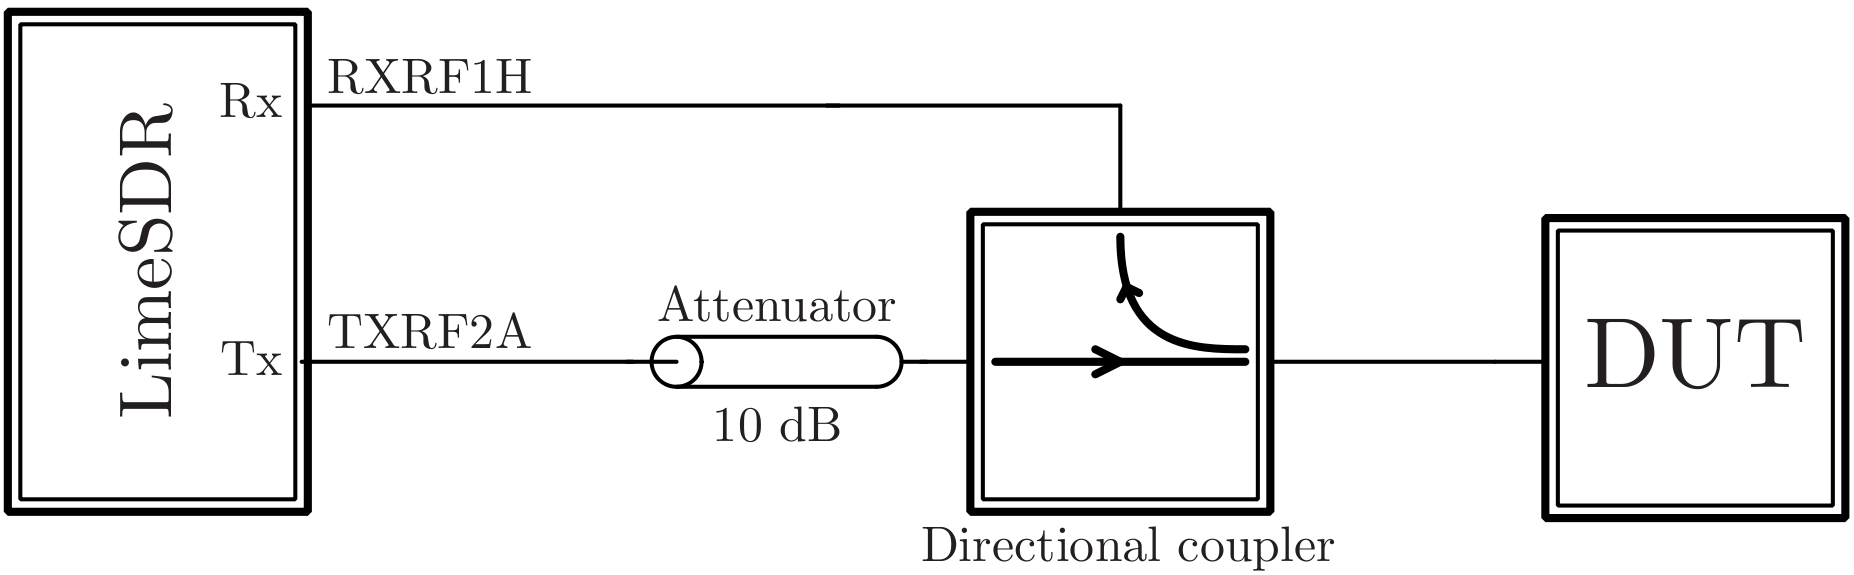
\includegraphics[scale=1]{demosetup}\\
   % translate x=408 y=390 scale 0.38
   \putbox{5.68in}{0.75in}{2.40}{\centbox{\midbox{DUT}}}%
   \putbox{3.79in}{0.09in}{1.20}{\centbox{Directional coupler}}%
   \putbox{0.54in}{1.09in}{1.80}{\rotatebox{-270}{\centbox{\midbox{LimeSDR}}}}%
   \putbox{0.97in}{0.75in}{1.20}{\rightbox{\midbox{Tx}}}%
   \putbox{0.97in}{1.61in}{1.20}{\rightbox{\midbox{Rx}}}%
   \putbox{2.62in}{0.89in}{1.20}{\centbox{Attenuator}}%
   \putbox{2.62in}{0.49in}{1.20}{\centbox{10 dB}}%
   \putbox{1.12in}{1.65in}{1.20}{RXRF1H}%
   \putbox{1.12in}{0.80in}{1.20}{TXRF2A}%
   } % close 'parbox'
   } % close 'scalebox'
   \vspace{-\baselineskip} % this is not necessary, but looks better
